\documentclass[11pt,dvipdfmx,b5paper,oneside,report,uplatex]{jsbook}


\usepackage{color}
\usepackage{here}
\usepackage{framed}
\usepackage{tcolorbox}
\usepackage{quotchap}
\usepackage{pdfpages}
\usepackage[hidelinks]{hyperref}
\usepackage{pxjahyper}
\usepackage{titlesec}
\usepackage{picture}
\usepackage{tikz}
\usepackage{graphicx}
\usepackage{geometry}
\usepackage{url}
\usepackage{pdfpages}


\tcbuselibrary{breakable,listings}
\definecolor{shadecolor}{gray}{0.80}

% 余白を狭くする
\geometry{left=20mm,right=20mm,top=25mm,bottom=25mm}

% section
\titleformat{\section}[block]{}{}{0pt}
{
  \definecolor{teal}{gray}{0.30}
  \begin{picture}(0,0)
    \put(-10,-5){
      \begin{tikzpicture}
        \fill[teal] (0pt,0pt) rectangle (5pt,19pt);
      \end{tikzpicture}
    }
    \put(-10,-5){
      \color{teal}
      \line(1,0){\hsize}
    }
  \end{picture}
  \hspace{0pt}
  \sf \Large \thesection
  \hspace{0pt}
}

% 図表見出し
\renewcommand{\tablename}{\textcolor{gray}{▼} 表}
\renewcommand{\figurename}{\textcolor{gray}{▲} 図}

\begin{document}

\begin{titlepage}
  \newgeometry{left=0cm,right=0cm,top=0cm,bottom=0cm}
  \centering
  \includepdf[pages={1},width=\paperwidth,height=\paperheight]{./image/01-title/outside.pdf}
  \restoregeometry % 元の余白に戻す
\end{titlepage}
%目次を自動的に作る。
\tableofcontents
\chapter{初めに}

さて、みなさん。Webサイトは作られていますか?
Webサイトを作る時にそのままHTMLを触ってGithubなどで管理をしてもいいのですが、やはりGithubを使ったことない人にとってはWebサイトの更新だけでかなり大変な作業になってしまいます。

そこで、今サークルの情報共有で用いているesaを用いてWebサイトを更新したら簡単に、誰でも更新できるのではないかと考え、実装してみることにしました。
そこまで難しくないので、ぜひ参考にしてみてください。
\chapter{実際の動作しているサイト}

現在、下記レポジトリ、サイトで実際に動作しています。
実際にesaから記事を取り出して、Githubにpushしているので、記事を更新するだけで、Webサイトが更新されます。


レポジトリ:
\url{https://github.com/SystemEngineeringTeam/BlogSiteMarkDown}

Webサイト:
\url{https://esa.harutiro.net/}

\begin{figure}[htbp]
  \begin{minipage}{0.5\hsize}
      \begin{center}
          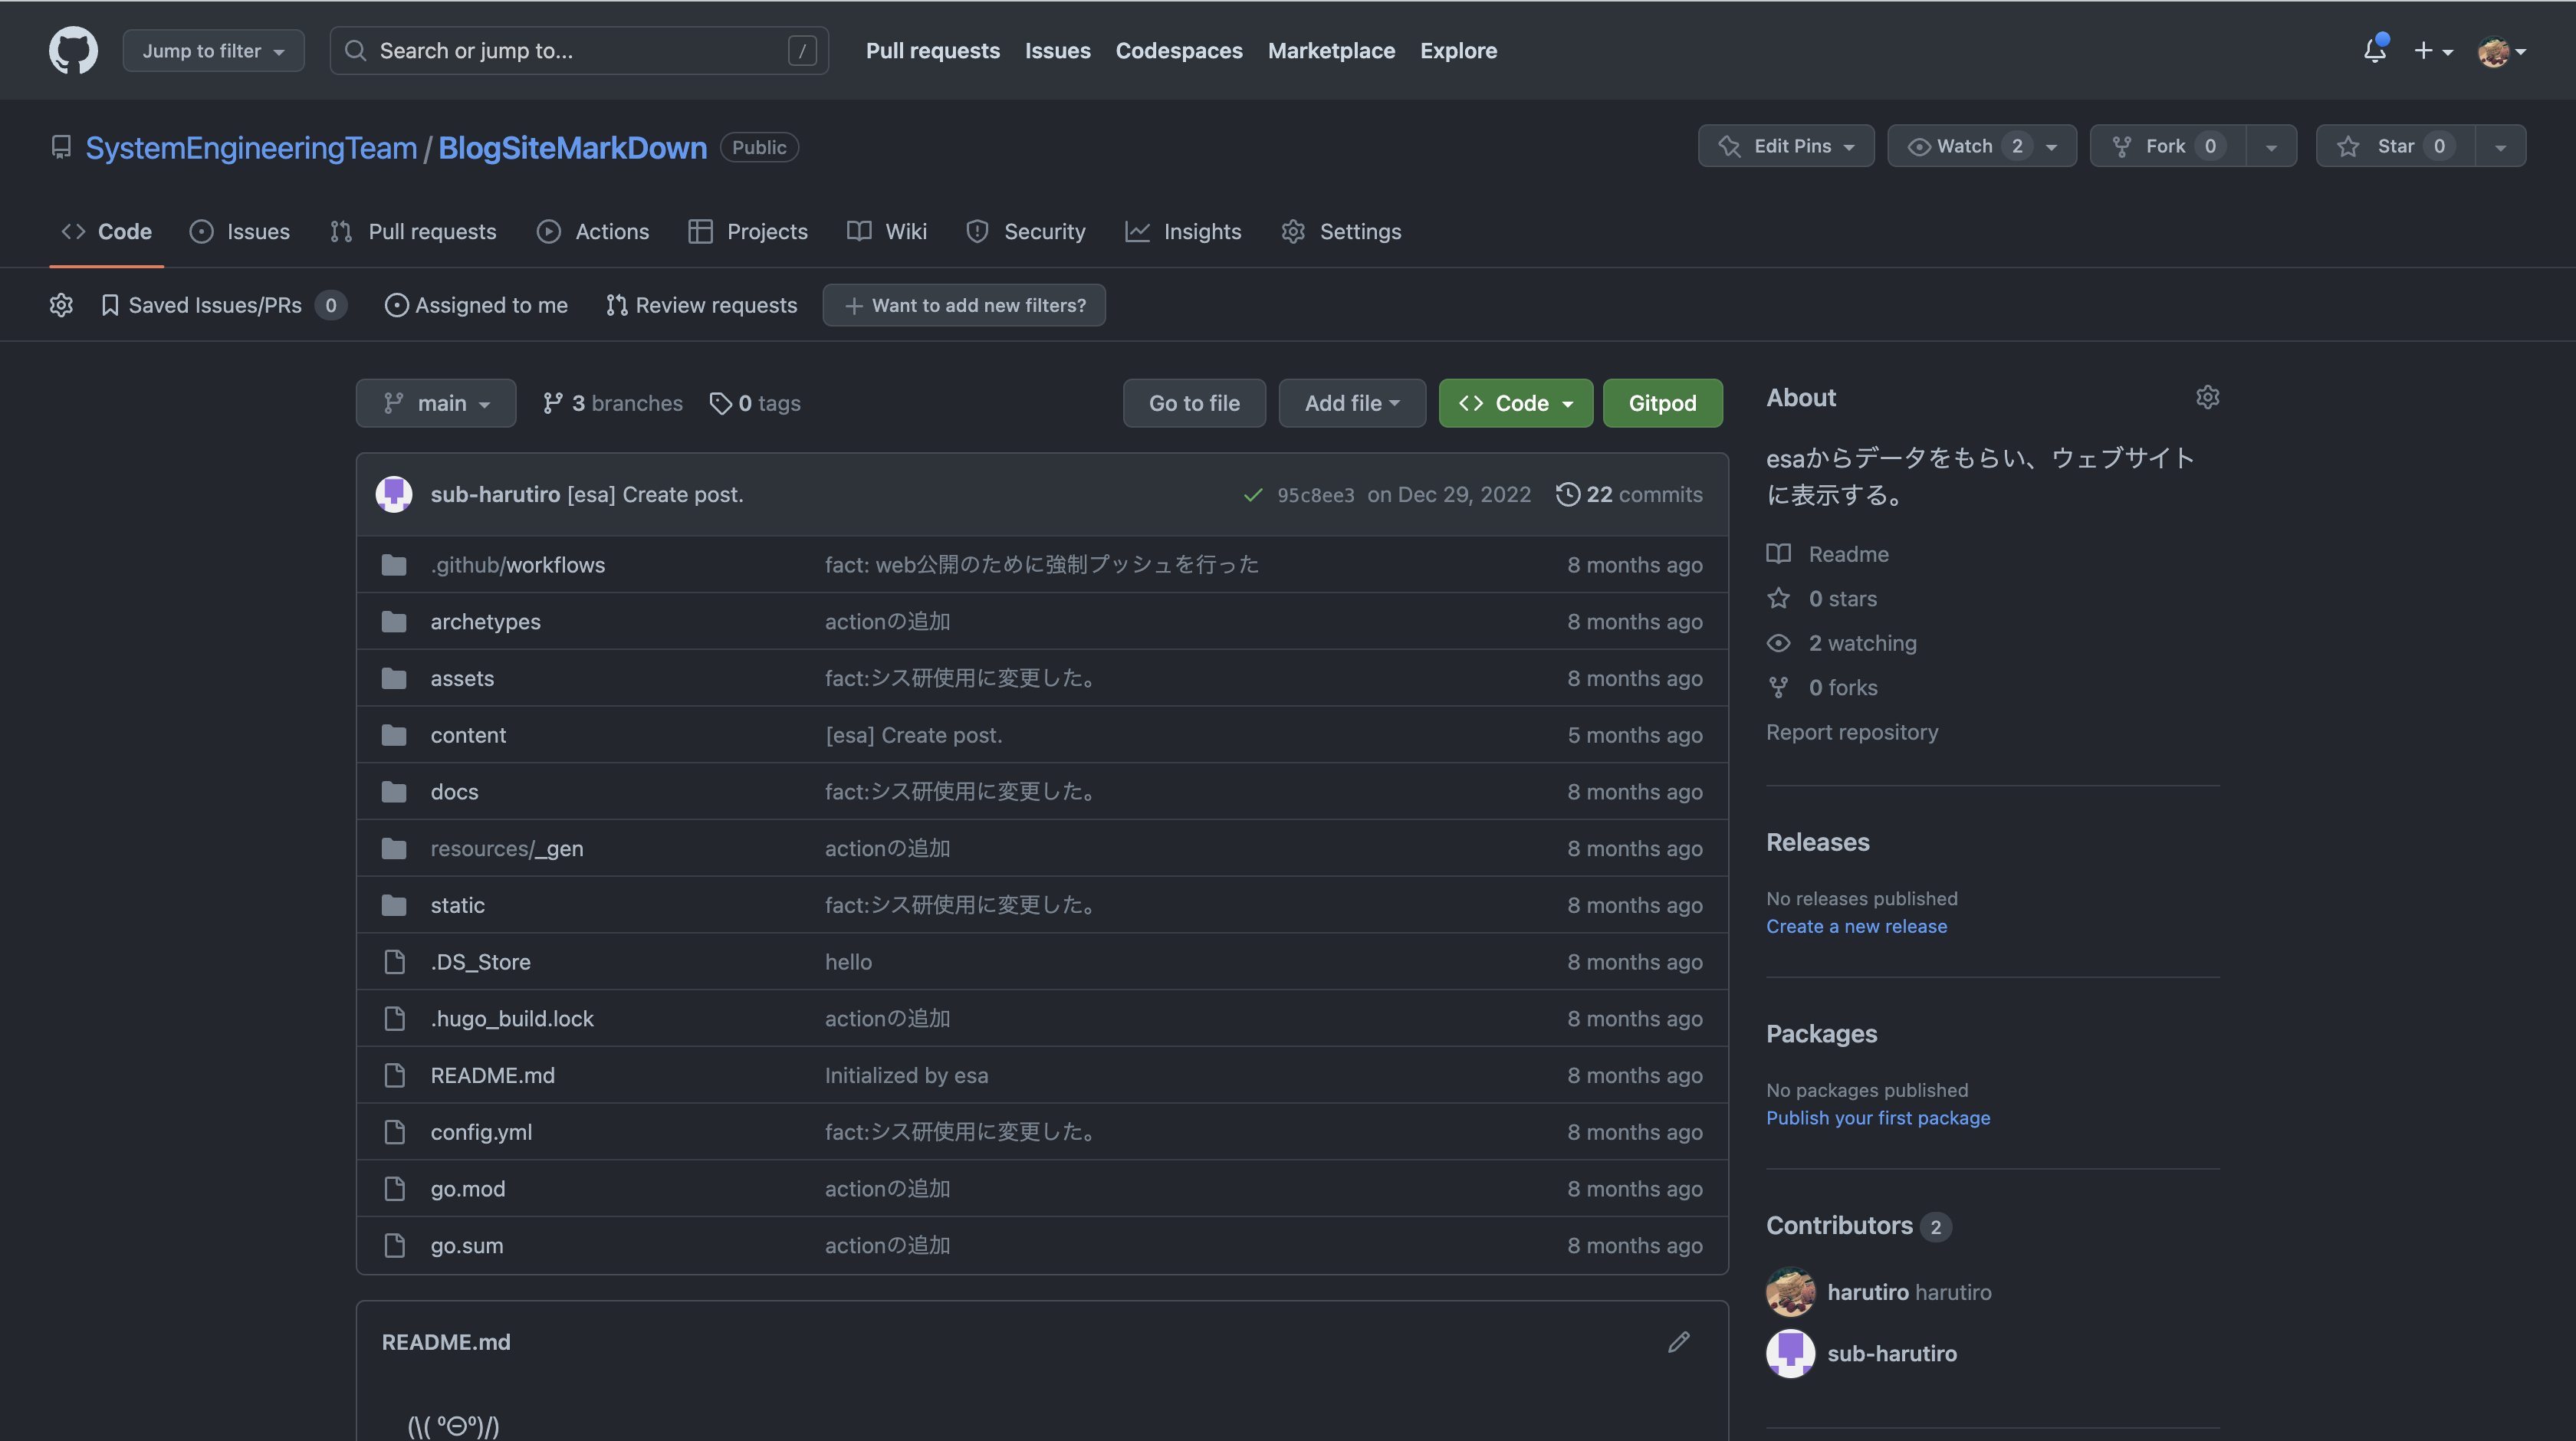
\includegraphics[width=50mm]{./image/02-chap2/git-repo.png}
      \end{center}
      \caption{Gitレポジトリ}
      \label{chap2-git-repo}
  \end{minipage}
  \begin{minipage}{0.5\hsize}
      \begin{center}
          
\includegraphics[width=50mm]{./image/02-chap2/sysken-web.png}
      \end{center}
      \caption{Webサイト}
      \label{chap2-web-site}
  \end{minipage}
\end{figure}
\chapter{用語まとめ}

\section{esa}

  \begin{figure}[H]
    \centering
    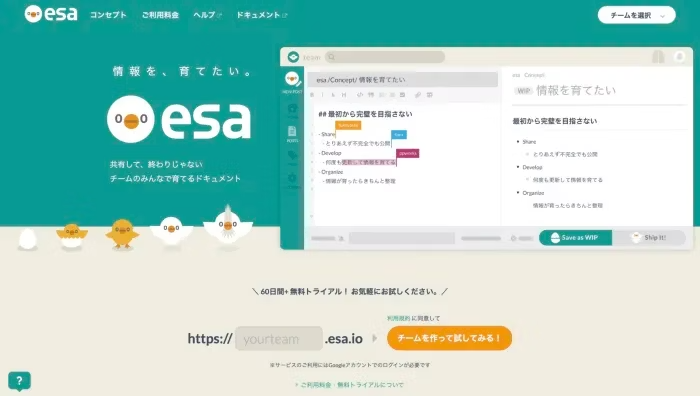
\includegraphics[width=6cm]{./image/02-chap3/esa.png}
    \caption{esaのホームページの写真}
    \label{chap3-esa-image}
  \end{figure}


  \begin{tcolorbox}[title=esaとは]
    esaとは、2014年に設立された合同会社esaの「情報共有ツール」です。
    esaは「不完全でも早い段階でチームに共有し、更新を重ねることでより良い情報に育つ」という発想のもと生まれました。そのため「Share(公開)」「Develop(更新して情報を育てる)」「Organize(育った情報を整理)」の3つの流れで設計されています。
    現在は3,000社を超える企業に導入されており、主に情報の蓄積やWIP機能(書いている途中でも共有する機能)を用いて、業務の効率化を実現している企業が多いです。
    \cite{esaとは} \cite{公式esaWeb}

  \end{tcolorbox}

\section{hugo}

  \begin{figure}[H]
    \centering
    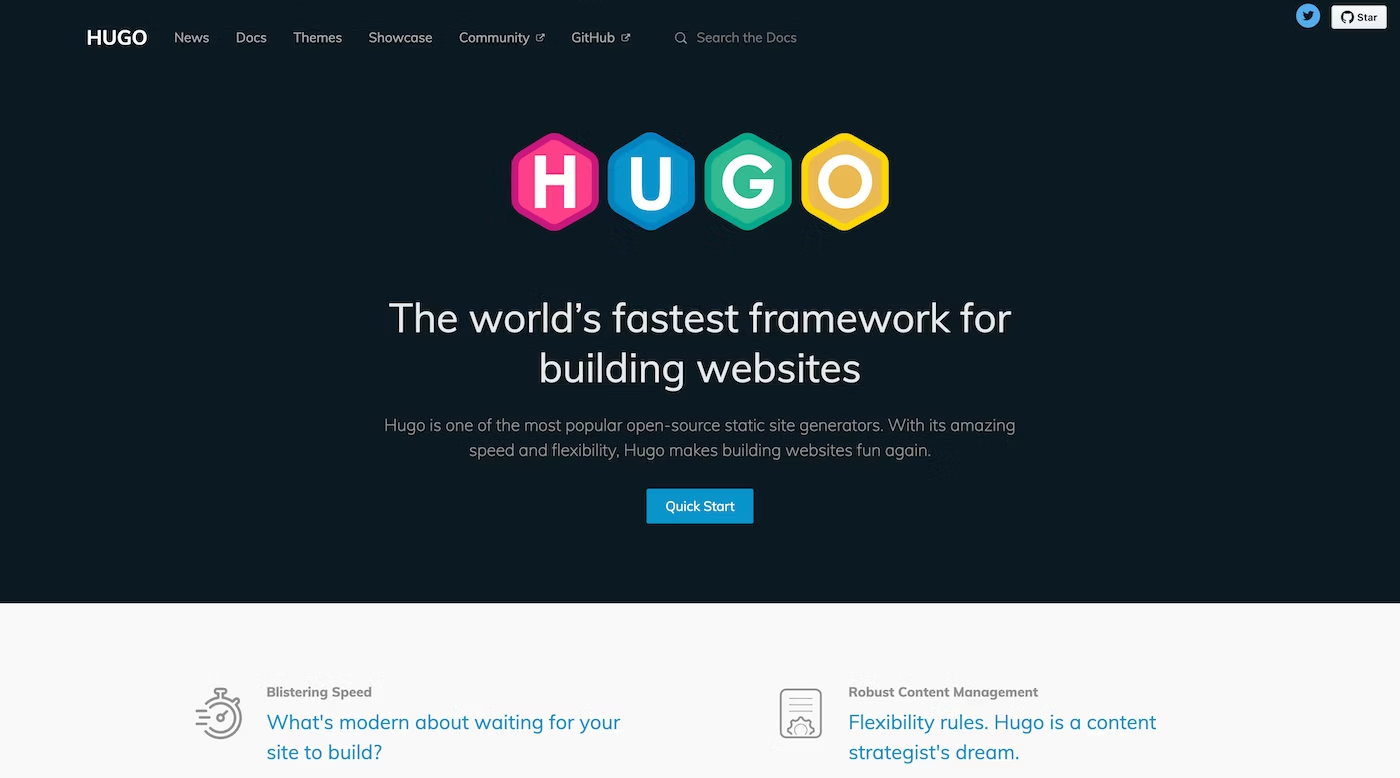
\includegraphics[width=6cm]{./image/02-chap3/hugo.png}
    \caption{hugoのホームページの写真}
    \label{chap3-hugo-image}
  \end{figure}

  \begin{tcolorbox}[title=hugoとは]
    HugoはGo言語で実装された「Webサイト構築フレームワーク」で、最初の公開は2013年という比較的新しいツールだ。コンテンツ管理システムではなく「Webサイト構築フレームワーク」と名乗っているとおり、コンテンツの管理ではなく、Webサイトで使われるHTMLファイルやRSSファイルなどの生成に特化した機能を備えている。
    \cite{hugoとは} \cite{hugo公式}
  \end{tcolorbox}

\section{GitHub Actions}

  \begin{figure}[H]
    \centering
    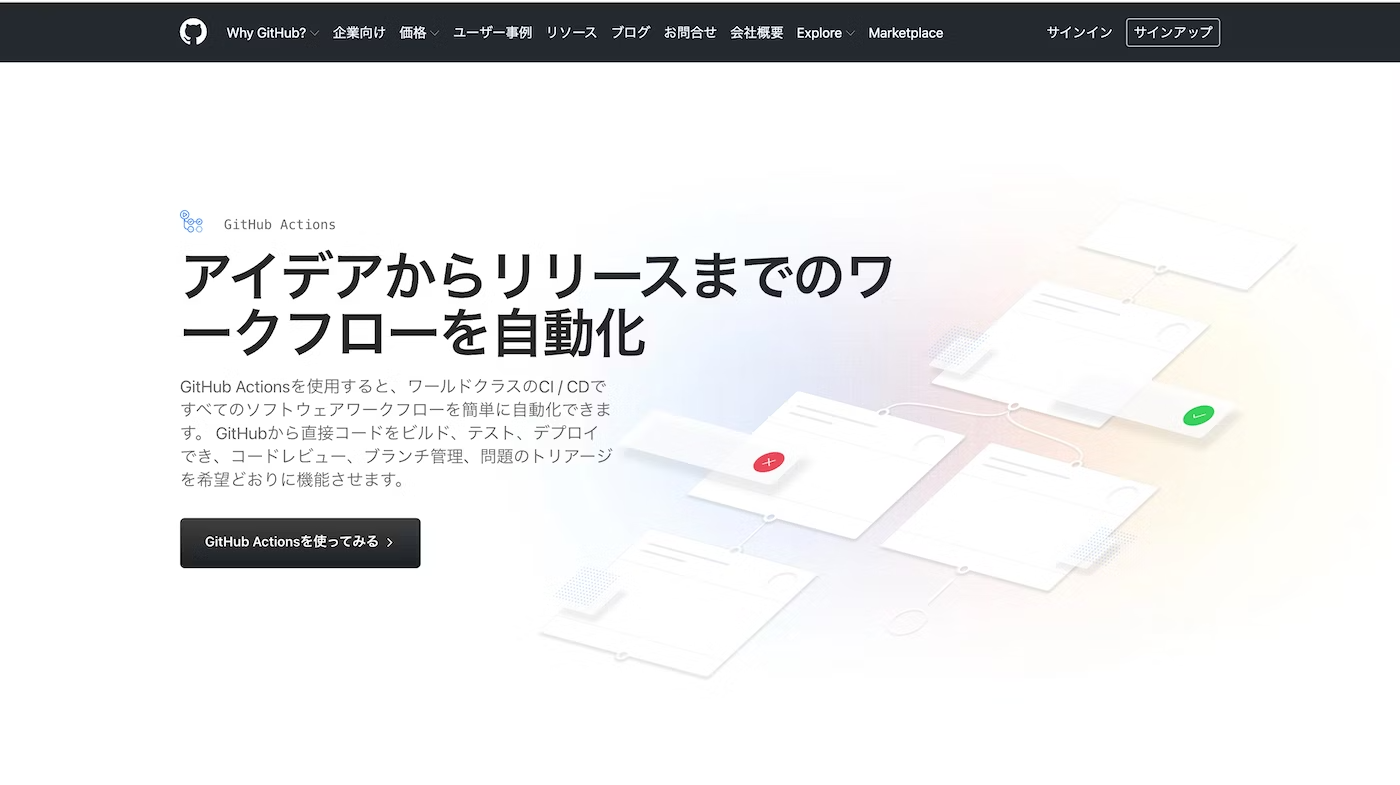
\includegraphics[width=6cm]{./image/02-chap3/githubActions.png}
    \caption{GitHub Actionsのホームページの写真}
    \label{chap3-githubAction-image}
  \end{figure}

  \begin{tcolorbox}[title=GitHub Pagesとは]
    GitHub Actionsで、ソフトウェア開発ワークフローをリポジトリの中で自動化し、カスタマイズし、実行しましょう。 CI/CDを含む好きなジョブを実行してくれるアクションを、見つけたり、作成したり、共有したり、完全にカスタマイズされたワークフロー中でアクションを組み合わせたりできます。
    \cite{githubAction}
  \end{tcolorbox}

\section{GitHub Pages}

  \begin{tcolorbox}[title=hugoとは]
    GitHub Pages は、GitHub のリポジトリから HTML、CSS、および JavaScript ファイル を直接取得し、任意でビルドプロセスを通じてファイルを実行し、ウェブサイトを公開できる静的なサイトホスティングサービスです。
    \cite{githubPages}
  \end{tcolorbox}


\section{CMS}

  \begin{tcolorbox}[title=CMSとは]
    「CMS」とは、「Contents Management System:コンテンツ・マネジメント・システム」の略で、簡単にいうとWebサイトのコンテンツを構成するテキストや画像、デザイン・レイアウト情報(テンプレート)などを一元的に保存・管理するシステムのことです。
    \cite{cmsとは}
  \end{tcolorbox}



\chapter{これはchapter}
\section{これはsection}
我輩は猫である\footnote{こんな感じで脚注を書く}。

どこで生れたかとんと見当がつかぬ。何でも薄暗いじめじめした所でニャーニャー泣いていた事だけは記憶している。吾輩はここで始めて人間というものを見た。しかもあとで聞くとそれは書生という人間中で一番獰悪な種族であったそうだ。この書生というのは時々我々を捕えて煮て食うという話である。

\begin{tcolorbox}[breakable]
\begin{verbatim}
1  /* ここにはソースコードを書く */
2  #include<stdio.h>
3
4  int main(void)
5  {
6    printf("Hello, World!\n");
7    return 0;
8  }
9  /* breakableを付けるとこんな感じで改行にも対応できる */
\end{verbatim}
\end{tcolorbox}

\begin{shaded}
\begin{verbatim}
## ここにはコマンドを書く
$ echo "Hello, World!"
\end{verbatim}
\end{shaded}

図表はキャプションを付けたときに、先頭に「▲」や「▼」を付けるようにした。

\begin{table}[H]
  \centering
  \caption{表のサンプル}
  \begin{tabular}{|c|l|l|l|} \hline
    日本 & hoge & fuga & piyo \\ \hline
    アメリカ & foo & bar & baz \\ \hline
  \end{tabular}
  \label{table-sample0402}
\end{table}

\begin{figure}[H]
  \centering
  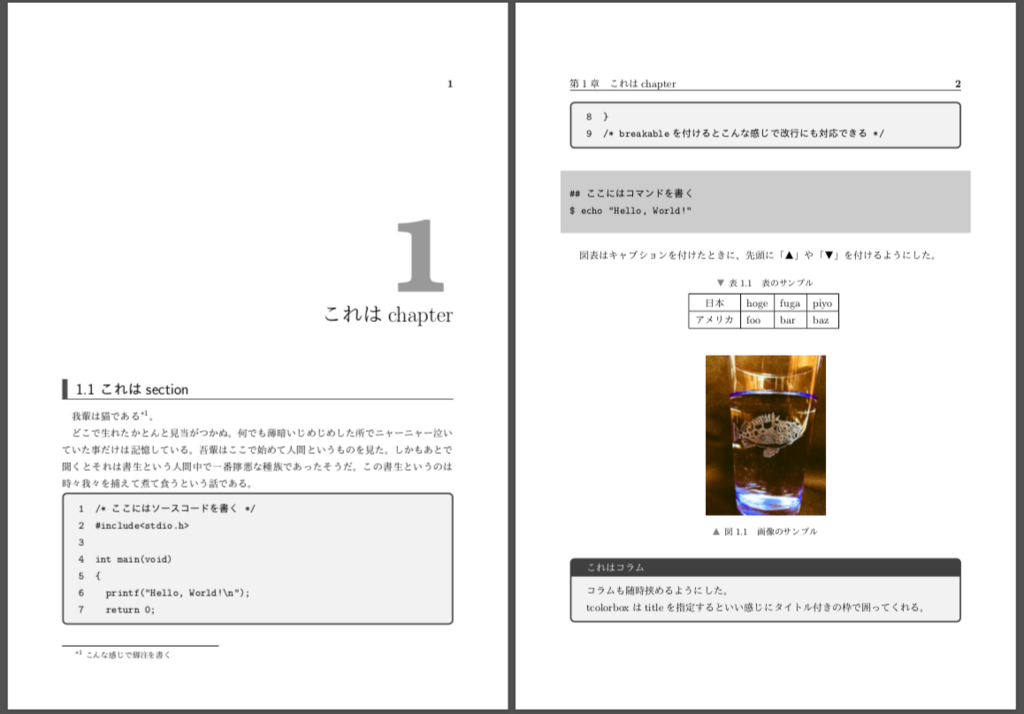
\includegraphics[width=4cm]{./image/sample.png}
  \caption{画像のサンプル}
  \label{figure-sample0402}
\end{figure}

\begin{tcolorbox}[title=これはコラム]
  コラムも随時挟めるようにした。

  tcolorboxはtitleを指定するといい感じにタイトル付きの枠で囲ってくれる。
\end{tcolorbox}






\end{document}